\documentclass[11pt, a4paper]{article}

\usepackage{graphicx}
\usepackage{forest}
\usepackage{proof}
\usepackage[utf8]{inputenc}
\usepackage{fancyhdr}
\usepackage{changepage}
\usepackage[onehalfspacing]{setspace}
\usepackage{ragged2e}
\usepackage{ amssymb, amsmath, amsthm, dsfont }
\usepackage[width = 18cm, top = 2.5cm, bottom = 3cm]{geometry}
\usepackage{extarrows}
\usepackage{stmaryrd}
% ---------

\newcommand{\myTitleString} {}
\newcommand{\myAuthorString} {}
\newcommand{\mySubTitleString} {}
\newcommand{\myDateString} {}

\newcommand{\myTitle}[1] {\renewcommand {\myTitleString}{#1}}
\newcommand{\mySubTitle}[1] {\renewcommand {\mySubTitleString}{#1}}
\newcommand{\myAuthor}[1] {\renewcommand{\myAuthorString}		{#1}}
\newcommand{\myDate}[1] {\renewcommand{\myDateString}{#1}}

\newcommand{\makeMyTitle}
{
\pagestyle{fancy}
\fancyhead[L]
{
\begin{tabular}{l}
\myTitleString
\\ \mySubTitleString 
\\ \myDateString
\end{tabular}
} 			
\fancyhead[C]{}
\fancyhead[R]{\myAuthorString}
\fancyfoot[C]{\thepage}
}

\setlength{\headheight}{45pt}

\newcommand{\p}{4}
\newcommand{\pp}{10}
\newcommand{\ppp}{8}
\newcommand{\pppp}{10} 

\newcommand{\defgl}{\mathrel{=\!\!\mathop:}}
\newcommand{\defgr}{\mathrel{\mathop:\!\!=}}

\makeatletter
\renewcommand*\env@matrix[1][*\c@MaxMatrixCols c]{%
  \hskip -\arraycolsep
  \let\@ifnextchar\new@ifnextchar
  \array{#1}}
\makeatother
% ---------
%\setlength{\parindent}{0pt}
\begin{document}

\myTitle{\textsc{Mathematische Logik}}
\mySubTitle{Übung 7}
\myDate{6. Juni 2017}
\myAuthor
{
\begin{tabular}{l l}
346532, &Daniel Boschmann\\
348776, &Anton Beliankou	\\
356092, &Daniel Schleiz
\end{tabular}
}
\makeMyTitle

\begin{tabular}{|c|c|c|c|c|}\hline
   2 & 3 & 4 & 5 &$\sum$\\\hline
  	 \qquad/\p & \qquad/\pp & \qquad/\ppp & \qquad/\pppp &\qquad/32\\\hline
 \end{tabular}
\hspace*{20pt} {\huge Gruppe \textbf{G}}
\vspace*{30pt}


\section*{Aufgabe 2 (Punkte:\qquad/\p)}
\textbf{(a)}
\begin{adjustwidth}{20pt}{20pt}
Wandle die Formel zunächst in PNF um.
\begin{align*}
	\varphi &= \forall x \exists yRxy \wedge (\neg Pz \vee \exists x\neg Rxy) \\
		&\equiv \forall x_1 \exists x_2Rx_1x_2 \wedge (\neg Pz \vee \exists x_3\neg Rx_3y)\\
		&\equiv \forall x_1 \exists x_2 \exists x_3(Rx_1x_2 \wedge(\neg Pz \vee \neg Rx_3y)) \in \text{FO}(\{ R,P\})
\end{align*}
Eliminiere nun schrittweise die Existenzquantoren, dabei entsteht jeweils eine neue Formel $\psi_i$.
\begin{align*}
	\psi_1 &= \forall x_1 \exists x_3(Rx_1fx_1 \wedge (\neg Pz \vee \neg Rx_3y))  \in \text{FO}(\{ R,P, f\}) \\
	\psi_2 &= \forall x_1(Rx_1fx_1 \wedge (\neg Pz \vee \neg Rgx_3y))  \in \text{FO}(\{ R,P,f,g\}) \\
\end{align*}
\end{adjustwidth}
\textbf{(b)}
\begin{adjustwidth}{20pt}{20pt}\vspace{-\baselineskip}
\begin{align*}
	\vartheta &= \forall x\exists y \forall z(\varphi \wedge \psi) \\
		&\equiv \forall x(\varphi \wedge \exists y \forall z \psi) \\
		&\equiv \forall x \varphi \wedge \forall x\exists y \forall z \psi \\
		&\equiv \forall x \varphi \wedge \exists y \forall z \psi \\
		&\equiv \forall x \varphi \wedge \exists y \forall z \forall x \psi \\
		&\equiv \exists y \forall z(\forall x \varphi \wedge \forall x \psi)i \\
		&\equiv \exists y\forall z \forall x(\varphi \wedge \psi)i \\
		&\equiv \exists y\forall x \forall z(\varphi \wedge \psi)
\end{align*}
\end{adjustwidth}


\section*{Aufgabe 3 (Punkte:\qquad/\pp)}
\textbf{(a)}
\begin{adjustwidth}{20pt}{20pt}

\end{adjustwidth}
\textbf{(b)}
\begin{adjustwidth}{20pt}{20pt}

\end{adjustwidth}
\textbf{(c)}
\begin{adjustwidth}{20pt}{20pt}

\end{adjustwidth}

\section*{Aufgabe 4 (Punkte:\qquad/\ppp)}
\textbf{(a)}
\begin{adjustwidth}{20pt}{20pt}\vspace{-\baselineskip}
\begin{align*}
\psi &= \forall x(\exists yExy \rightarrow \exists z(Exz \wedge Ezz)) \\
	&\equiv \forall x(\neg(\exists yExy) \vee \exists z(Exz \wedge Ezz)) \\
	&\equiv \forall x(\forall y\neg Exy \vee \exists z(Exz \wedge Ezz))
\end{align*}
\end{adjustwidth}
\textbf{(b)}
\begin{adjustwidth}{20pt}{20pt}
Seien $\eta = \forall y\neg Exy \vee \exists z(Exz \wedge Ezz)$, $\psi = \forall y\neg Exy$, $\vartheta = \exists z(Exz \wedge Ezz)$ und $\phi = Exz \wedge Ezz$.
\begin{figure}[h]
\centering
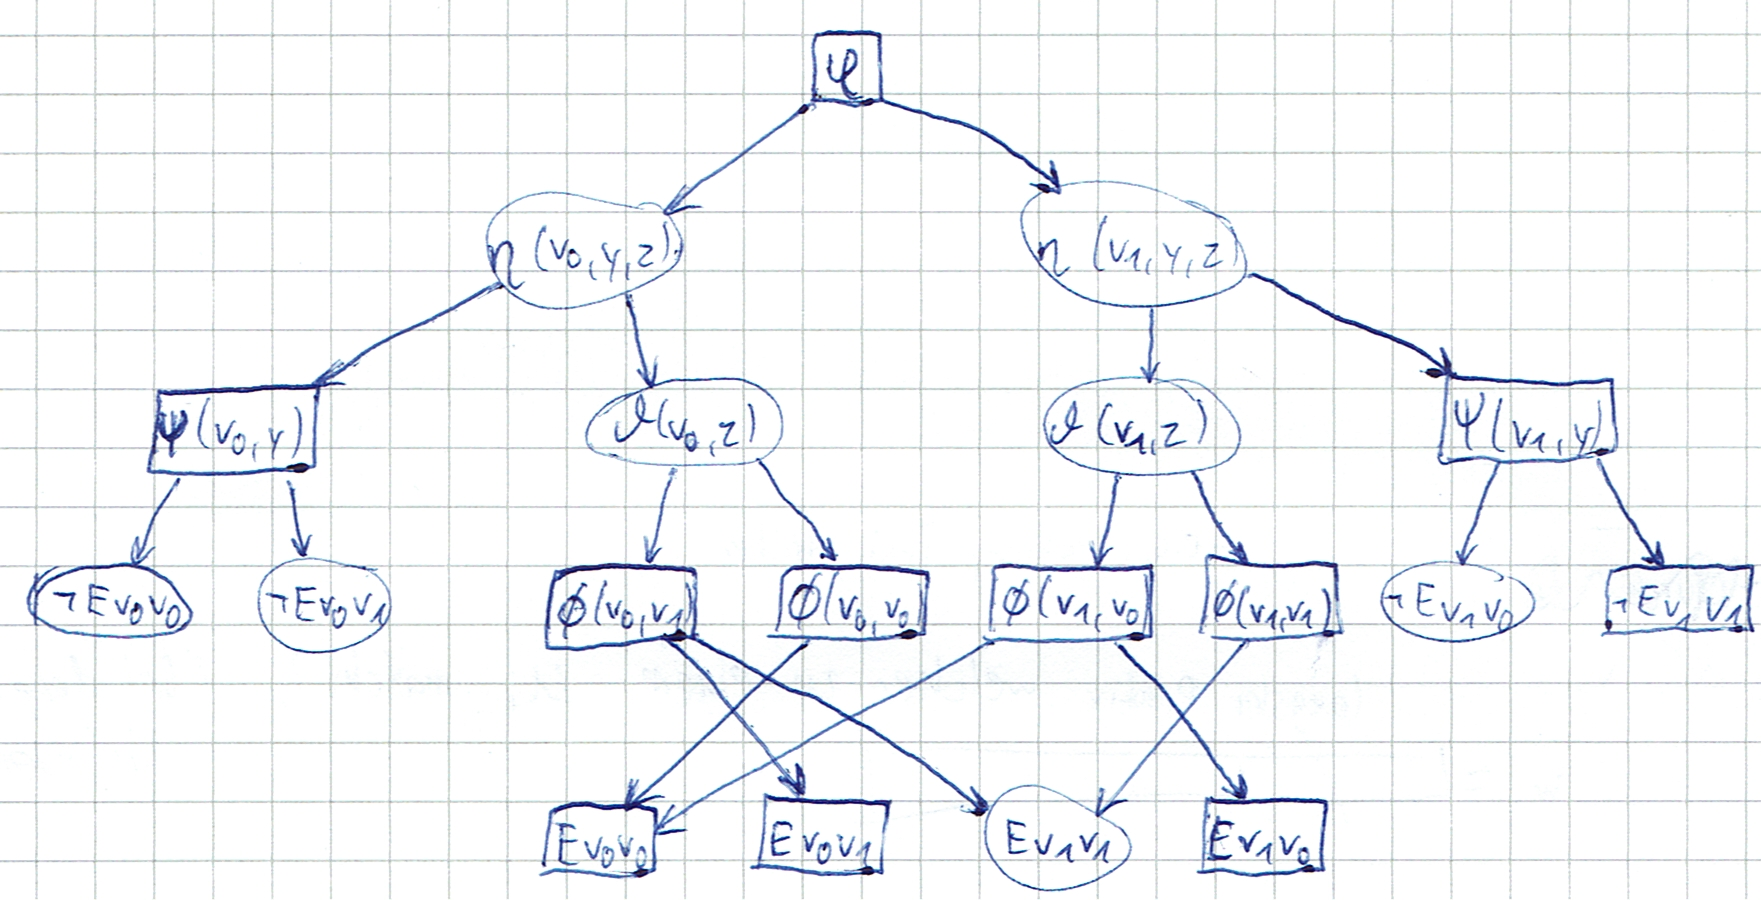
\includegraphics{4b.png}
\end{figure}\\
(Positionen, welche aus verschiedenen Teilformeln entstehen würden, jedoch syntaktisch die gleiche Formel darstellen, wurden als Knoten der Übersichtlichkeit halber zusammengefasst.
[Betroffen sind nur Knoten, die Kanten darstellen, auf der untersten "Ebene".])\\
Es existiert eine Gewinnstrategie $f$ für die Verifiziererin von der Startposition aus, welche wie folgt definiert ist:
\begin{itemize}
\item $f(\eta(v_i,y,z))=\vartheta(v_i,z)$ mit $i \in \{ 1,2\}$
\item $f(\vartheta(v_i,z))= \phi(v_i,v_o)$ mit $i \in \{ 1,2\}$
\end{itemize}
Dabei handelt es sich um eine Gewinnstrategie, zunächst kein Knoten ohne Nachfolger existiert, weshalb stets die $\vartheta$-Teilformel gewählt werden muss, und anschließend stets
$z=v_0$ gewählt werden kann, da $Ev_iv_0$ wahr ist und ebenfalls $Ev_0v_0$ wahr ist. 
\end{adjustwidth}


\section*{Aufgabe 5 (Punkte:\qquad/\pppp)}
Die folgenden FO-Formeln sind über der Signatur $\{ V_0,V_1,E\}$ über dem Universum $V$ definiert. \\
\textbf{(a)}\\
\textbf{(i)}\vspace{-\baselineskip}
\begin{adjustwidth}{20pt}{20pt}
$\varphi_i(v)\defgr \forall x(Evx \rightarrow \forall y(Exy \rightarrow \neg\exists zEyz))$\\
Für alle Nachfolger $x$ von $v$, falls welche existieren, müssen wiederum alle Nachfolger $y$ von $x$, falls diese existieren, eine Endposition sein.\\
\end{adjustwidth}
\textbf{(ii)}\vspace{-\baselineskip}
\begin{adjustwidth}{20pt}{20pt}
$\varphi^n_{ii}(v,w)\defgr \Big((V_1v \rightarrow \forall x(Evx \rightarrow \varphi^{n-1}_{ii}(x,w))) \wedge (V_0v \rightarrow \exists y(Evy \rightarrow \varphi^{n-1}_{ii}(y,w)))\Big) \vee v=w$ und definiere
noch zusätzlich $\varphi^0_{ii}(v,w) \defgr v = w$.\\
Idee: Falls $v$ in $V_1$ liegt (und somit Spieler 1 zieht), muss für alle Nachfolger die Formel mit $n-1$ gelten, da $V_1$ den Nachfolger wählen darf und somit ein Schritt "verbraucht" wird.
Ist aber $V_0$ am Zug, so muss die Formel nur für einen Nachfolger mit $n-1$ gelten, da Spieler 0 wählen kann. Da die Forderung höchstens $n$ Schritte ist, ist die Formel auch erfüllt, falls
$v=w$. Für ein festes $n$ lässt sich die Formel aufgrund des eindeutigen Rekursionsschlusses bei 0 komplett ausschreiben, weshalb eine FO-Formel vorliegt. Somit definiert die Formel
gerade die geforderte Relation. 
\end{adjustwidth}
\textbf{(b)}
\begin{adjustwidth}{20pt}{20pt}
Definiere zunächst die Teilformel $\psi_L(v)$, welche ausdrücken soll, dass Spieler 0 von $v$ aus keine Gewinnstrategie hat:\\
$\psi_L(v) \defgr \forall x(V_1x \wedge \neg\exists yExy \rightarrow \neg\varphi^n_{ii}(v,x) )$\\
Die Formel besagt also, dass alle Knoten, bei welchen Spieler 1 ziehen müsste und die keine Nachfolger haben, nicht von $v$ aus von Spieler 0 in höchstens $n$ Schritten erzwungen werden
können. Es reicht dabei, Pfade der Länge höchstens $n$ zu betrachten, da der Graph nur aus $n$ Knoten besteht und somit jeder Knoten, welcher von Spieler 0 von $v$ aus erzwungen
werden kann, ebenfalls in höchstens $n$ Schritten erzwungen werden kann, da man höchstens den ganzen Graphen traversiert und Kreise im "Pfad" weglassen kann.\\ \ \\
Definiere nun die Teilformel $\psi_\infty(v)$, welche ausdrückt, dass Spieler 0 von $v$ aus eine unendliche Partie erzwingen kann:\\
$\psi_\infty(v) \defgr \exists x(\varphi^n_{ii}(v,x) \wedge \exists y(y \neq x \wedge \varphi^n_{ii}(x,y) \wedge \varphi^n_{ii}(y,x)))$\\
Die Formel ist wahr, falls ein Knoten $x$ existiert, sodass Spieler 0 diesen Knoten von $v$ aus erzwingen kann und sodass man einen Pfad von $x$ zu $x$ erzwingen kann über einen
anderen Knoten $y$. Dies entspricht gerade der Möglichkeit, eine unendliche Partie zu erzwingen, da Spieler 0 dann unendlich oft $x$ zu $x$ erzwingen kann. Es genügt ebenfalls
aus analogen Gründen wie in der ersten Teilformel, erzwungene Pfade der Länge höchstens $n$ zu betrachten. Es ergibt sich nun die Gesamtformel\\
$\psi_{L\infty}(v) \defgr \psi_L(v) \wedge \psi_\infty(v)$
%$\psi_n(v)\defgr$
\end{adjustwidth}

\end{document}
